\subsection{固定条件问题中可以直接使用的性质}

单教师的幂均值框架提供了三个相互连接的保证。正形状 $\kappa>0$ 改变极端教师概率比的尾部；固定 $(\kappa,\eta)$ 的精确更新下降一个明确的有界教师目标 $\mathcal J$；$0<\kappa\le1/2$ 的中心化监督方差又由中心 $K$ 控制。BPO 拟合的残差采样梯度随其损失下降而消失，形状变换与残差回归分别控制初始监督和拟合末期的噪声。

\begin{center}
\small
\begin{tabular}{p{46mm}p{54mm}p{45mm}}
\toprule
可用性质 & 必要条件 & 实际含义\\
\midrule
精确 target 同时改善全部凸 $f$ 散度 & 同一固定 teacher、完整正支持 & 同一评价量下可比较不同形状\\
教师覆盖与刷新后的双侧监督界 & $\kappa>0$，同一前缀精确刷新 & $q_n\ge\eta^{1/\kappa}T$，控制未来正尾部\\
精确 MD 下降与最后迭代界 & 固定 $\kappa,\eta$，每步刷新锚点 & $\mathcal J(q_N)\le\KL(T\Vert q_0)/(\eta N)$\\
教师监督方差受误差控制且可求和 & $0<\kappa\le1/2$，精确外层 & 教师接近度与监督噪声共同趋零\\
BPO 的零残差零采样梯度 & target 可实现、精确中心或无偏差分损失 & 避免固定中心误差造成的噪声底\\
有限 inner 的全部 teacher 散度进展 & 从 $q$ 出发的指定 Fisher 预条件路径 & 实际任意 BPO loss 下降不充分\\
有界中心估计与可认证尾部误差 & 已知 $q,T$ 概率或所需尾部查询接口 & 不增加 response 数仍可估计中心\\
\bottomrule
\end{tabular}
\end{center}

以上几何重心与球面性质属于已有信息几何框架；本章不据此宣称研究新颖性。本章用于 MirrorOPD 的增量在于明确分开重心、有限步 MD 目标、BPO 投影和估计器，并把它们连接为条件进展与噪声界。任务表现仍受共享参数、不可实现 target、有限 inner 和前缀访问变化影响。理论上可证明的对象与需要实测的对象在表中分别列出。

\subsection{原始几何信号的尺度与标准化反例}

在前八章的归一化下，记 $r=\log(T/q)$、$U=\log(p/q)$、$\psi=\nabla\log p$，三个原始下降方向为
\begin{align}
 -\nabla\mathcal L_{\mathrm{Mean}}&=\E_q[(\eta C_qr-U)\psi],\\
 -\nabla\mathcal L_{\mathrm{BPO}}&=\E_q[(C_qr-C_qU/\eta)\psi],\\
 -\nabla\mathcal L_{\mathrm{MDPO}}&=\E_p[(r-U/\eta)\psi].
\end{align}
在 $p=q$ 时，PMD-Mean 起始梯度带整体 $\eta$，BPO 与 MDPO 不带。第~\ref{sec:power-setup}~节二元反例中，未中心化的 MDPO 单点估计还满足
\begin{equation}
 \Var_q(\psi r)=v(1-v)[(1-v)r_1+vr_2]^2\longrightarrow\infty.
\end{equation}
这些尺度差异由具体损失归一化决定，不能仅由 target 的插值权重推断。

对二元信号 $f$，条件标准差为 $\sigma_f^2=v(1-v)(f_1-f_2)^2$。只要 $f_1\ne f_2$，逐 action 展开可得
\begin{equation}
 \Var_q[\psi C_qf/\sigma_f]=(1-2v)^2.
\end{equation}
单调信号变换在这个例子中被标准差缩放抵消。当前算法不使用这类随机标准差归一化；该反例用于限定原始方差界的适用对象。

\begin{figure}[htbp]
 \centering
 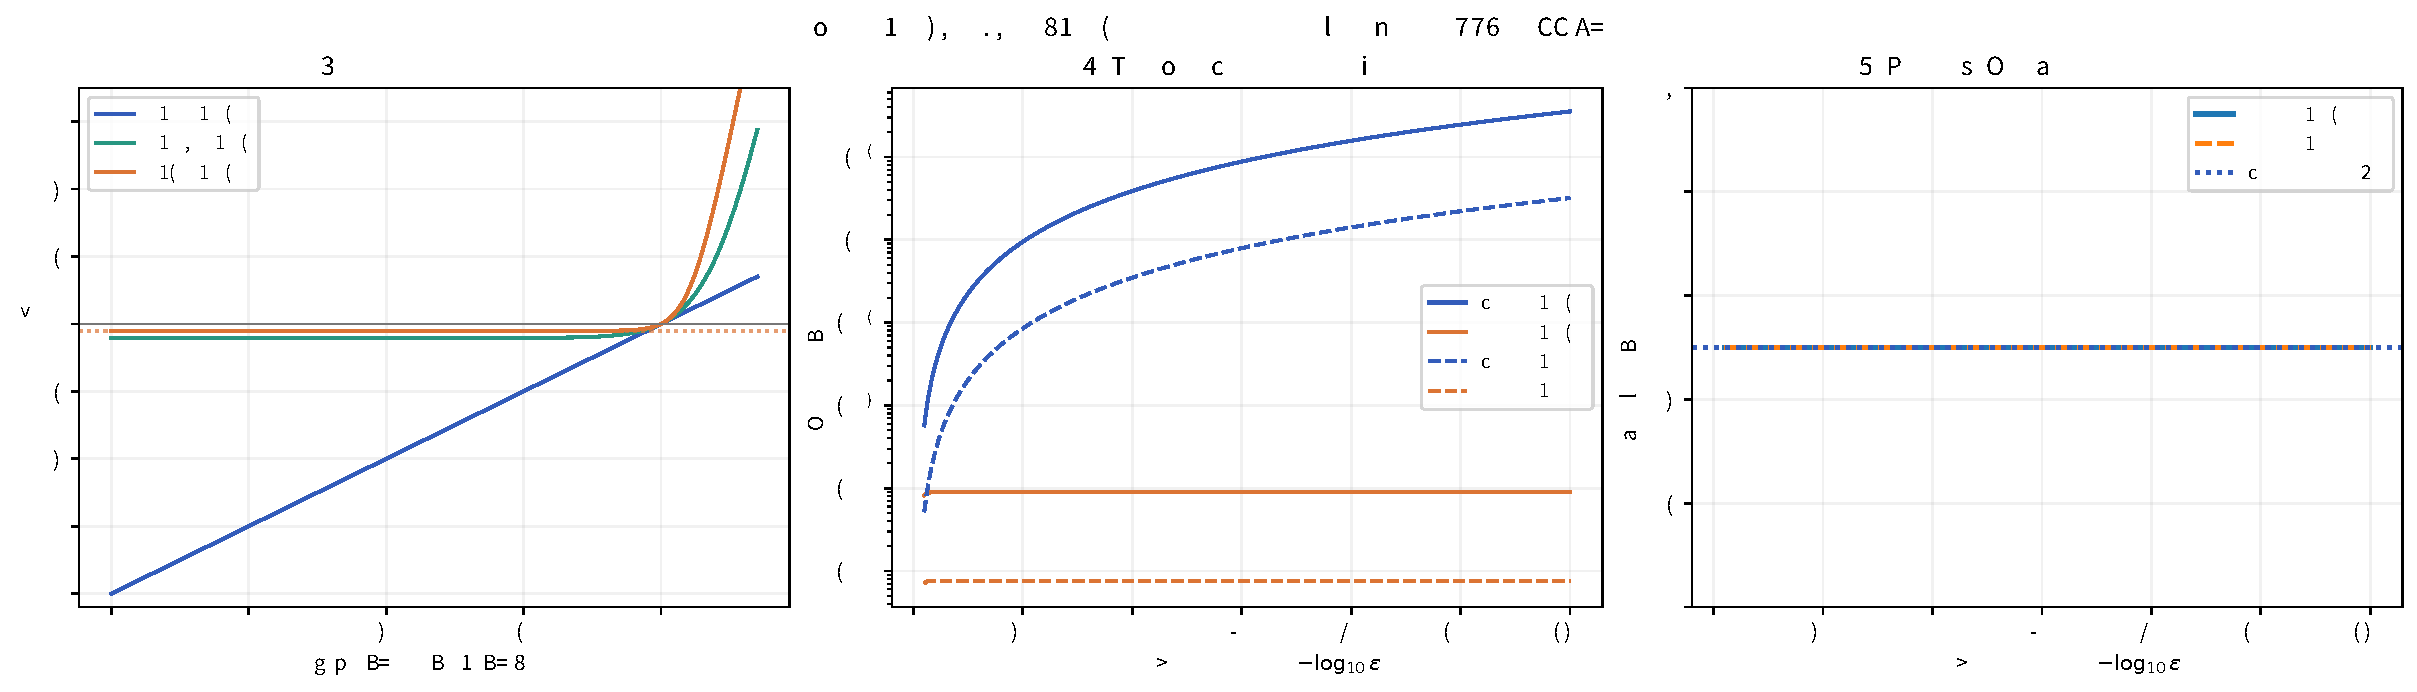
\includegraphics[width=\textwidth]{../../results/proximal-family-geometry/variance.pdf}
 \caption{尺度、尾部与标准化分别改变不同对象。早期图中 $\lambda$ 对应本章 $\eta$；中图使用 $q=(1/4,3/4)$ 的精确条件中心化 score 方差，右图验证二元标准差缩放的抵消现象。}
\end{figure}

\subsection{证明、解析图与实验记录的维护位置}

本章的图来自解析有限词表公式、已有模型缓存或已经登记的实验；正文与图注明确区分这些证据。重构只增加解析形状与反例图，不启动新的 GPU 训练。主线的 source、figure metadata 和确定性数值核验分别保存在 \path{docs/book/}、\path{results/chapter9-restructure/} 与对应第一方程序中。

原有几何、动力学和共享参数核验由 \path{experiments/analysis/proximal_family_geometry.py}、\path{experiments/analysis/proximal_family_dynamics.py} 生成。散度证书由 \path{experiments/analysis/power_generalization.py} 核验。中心和辅助采样的缓存审计位于 \path{results/power-center-advantage/} 与 \path{results/power-center-extensions/}。实际大模型 setting、结果和分析继续进入唯一实验报告，本章不复制待执行的 GPU 队列和运行流水。
